
\centerline{\textbf{ \LARGE Paging}}


% ----------------------------------------------------------------------------


\begin{enumerate}

  \begin{figure}[h]
      \centering   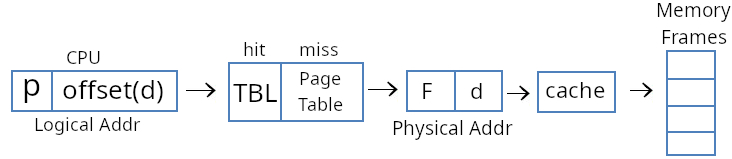
\includegraphics[scale=2.5]{./images/paging_01.jpeg}
  \end{figure}
  \item Paging \\
  \begin{myTableStyle}
    \begin{tabular}{ |m{3.5cm}|m{10cm}| } \hline
        Frame           &     Physical Address Space divided into frames                  \\ \hline
        Page            &     Logical   Address Space divided into pages.                 \\
                        &     Page size defined by hardware                               \\ \hline
        Page Table      &     maping of page no to frame no                               \\ \hline
        Word            &     Page Size = Frame Size =  \(2^k\) words                     \\ \hline
        offset(k-bits)  &     index of the word in a page/frame  \\ \hline
        Logical address &     page no(p)  +  offset(d)                                    \\ \hline
        Physical address&     frame no(f) +  offset(d)                                    \\ \hline
        Page Table Size &     \(2^p\) x size of one entry                                       \\
                        &     \(2^p\) = No of entries in page table = total pages                \\ \hline
        Translation \mbox{Lookaside} Buffer(TLB) & Acts as cache for page table                    \\ \hline
    \end{tabular}
  \end{myTableStyle}
  \vspace{0.08in}

  \item Each process has a page table.
  \item PT can not be in registers because registers are small in size.
  \item PT are kept in memory. Two main memory references are required to access a word in memory.
  \item Page table entry (PTE) \\
  \begin{myTableStyle}
    \begin{tabular}{ |m{2cm}|m{2cm}|m{2cm}|m{2cm}|m{3cm}| } \hline
        Page no &  Frame no & Valid bit & Dirty bit & Protection bit  \\ \hline
    \end{tabular}
  \end{myTableStyle}


  \item TLB : https://www.geeksforgeeks.org/translation-lookaside-buffer-tlb-in-paging/
    \begin{enumerate}
      \item Is a high-speed cache that stores a part of page table(PT).
      \item TLB miss : TLB is updated with new PTE.
      \item TLB entry replacement policies : FIFO, LRU or MFU etc
      \item TLB first checks. If the page is not in memory a page fault is issued then the TLB is updated to include the new page entry.
    \end{enumerate}

    \item Page sharing : multiple processes share the same  frame. Each PT will have an PTE for that frame.

  \item Two-Level Paging Example
  \begin{enumerate}
    \item  A logical address (on 32 -bit machine with 1 K page size) is divided into:
    \begin{enumerate}
      \item a page number consisting of 22 bits
      \item a page offset consisting of 10 bits
    \end{enumerate}
    \item Since the page table is paged, the page number is further divided into:
    \begin{enumerate}
        \item a 12 -bit page number
        \item a 10 -bit page offset
    \end{enumerate}
  \item Thus, a logical address is as follows:
    \begin{figure}[h]
        \centering   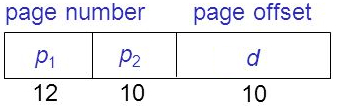
\includegraphics[scale=2.5]{./images/paging_02.jpeg}
    \end{figure}
  \item where pi is an index into the outer page table, and p 2 is the displacement within the page of the outer page table.
  \item Known as forward-mapped page table.
  \end{enumerate}

\end{enumerate}

% ----------------------------------------------------------------------------

% ----------------------------------------------------------------------------

% ----------------------------------------------------------------------------

% ----------------------------------------------------------------------------

% ----------------------------------------------------------------------------

% ----------------------------------------------------------------------------

% ----------------------------------------------------------------------------

% ----------------------------------------------------------------------------
